\documentclass[aps, prc, 12pt, nofootinbib, showpacs, superscriptaddress, tightenlines, groupedaddress]{revtex4-2}
\usepackage{amsmath,amssymb,amsbsy,bm}
\usepackage{graphicx}
\usepackage{comment}
\usepackage{float}
\usepackage[colorlinks=true,linkcolor=blue,citecolor=blue,urlcolor=blue]{hyperref}
\usepackage[margin=0.75in]{geometry}
\usepackage{silence}
\WarningFilter{revtex4-2}{Repair the float}

%\usepackage[table]{xcolor}

\begin{document}

\title{Charge balance functions for heavy-ion collisions at energies
   available at the CERN Large Hadron Collider}
\author{Scott Pratt}
\affiliation{Department of Physics and Astronomy and National Superconducting Cyclotron Laboratory\\
Michigan State University, East Lansing, MI 48824~~USA}
\date{\today}

\pacs{}

\begin{abstract}
baryon transport ...
\end{abstract}

\maketitle

\section{Introduction}

\section{Baryon Transport from Merging Simple Flux Tubes}

Here, we consider the merging of two simple flux tubes into one. The term ``simple'' refers to the fact that the tube is generated by a single quark or anti-quark. In a simple tube, one can bisect the tube at any point and classify the color charge on each side of the bisection by its color multiplet, $p,q$. In SU(3), the multiplet is defined by two integers, which differs from SU(2), where a multiplet is denoted by a single number, $j$, e.g. the total angular momentum. Graphically, the state can be enumerated by the graphs in Fig. \ref{fig:pqmultiplet}. Multiplets denoted by $(p_1,q_1)$ and $(p_2,q_2)$ can be combined to create multiplets denoted by $(p',q')$. In SU(2), multiplets denoted by $j_1$ and $j_2$ only couple to singlet $j'=0$ if $j_1=j_2$. Similarly, for SU(3) two multiplets couple to a color singlet only if $p_1=q_2$ and $p_2=q_1$. For example, the $(1,0)$ multiplet (quark) and the $(0,1)$ multiplet (antiquark) can couple to a color singlet.

Before addressing merging, we review the case of a simple flux tube between a quark and antiquark. Figure \ref{fig:simpletube} illustrates how the flux can be reduced by quark-antiquark pairs tunneling out of the vacuum. 
\begin{figure}
\centerline{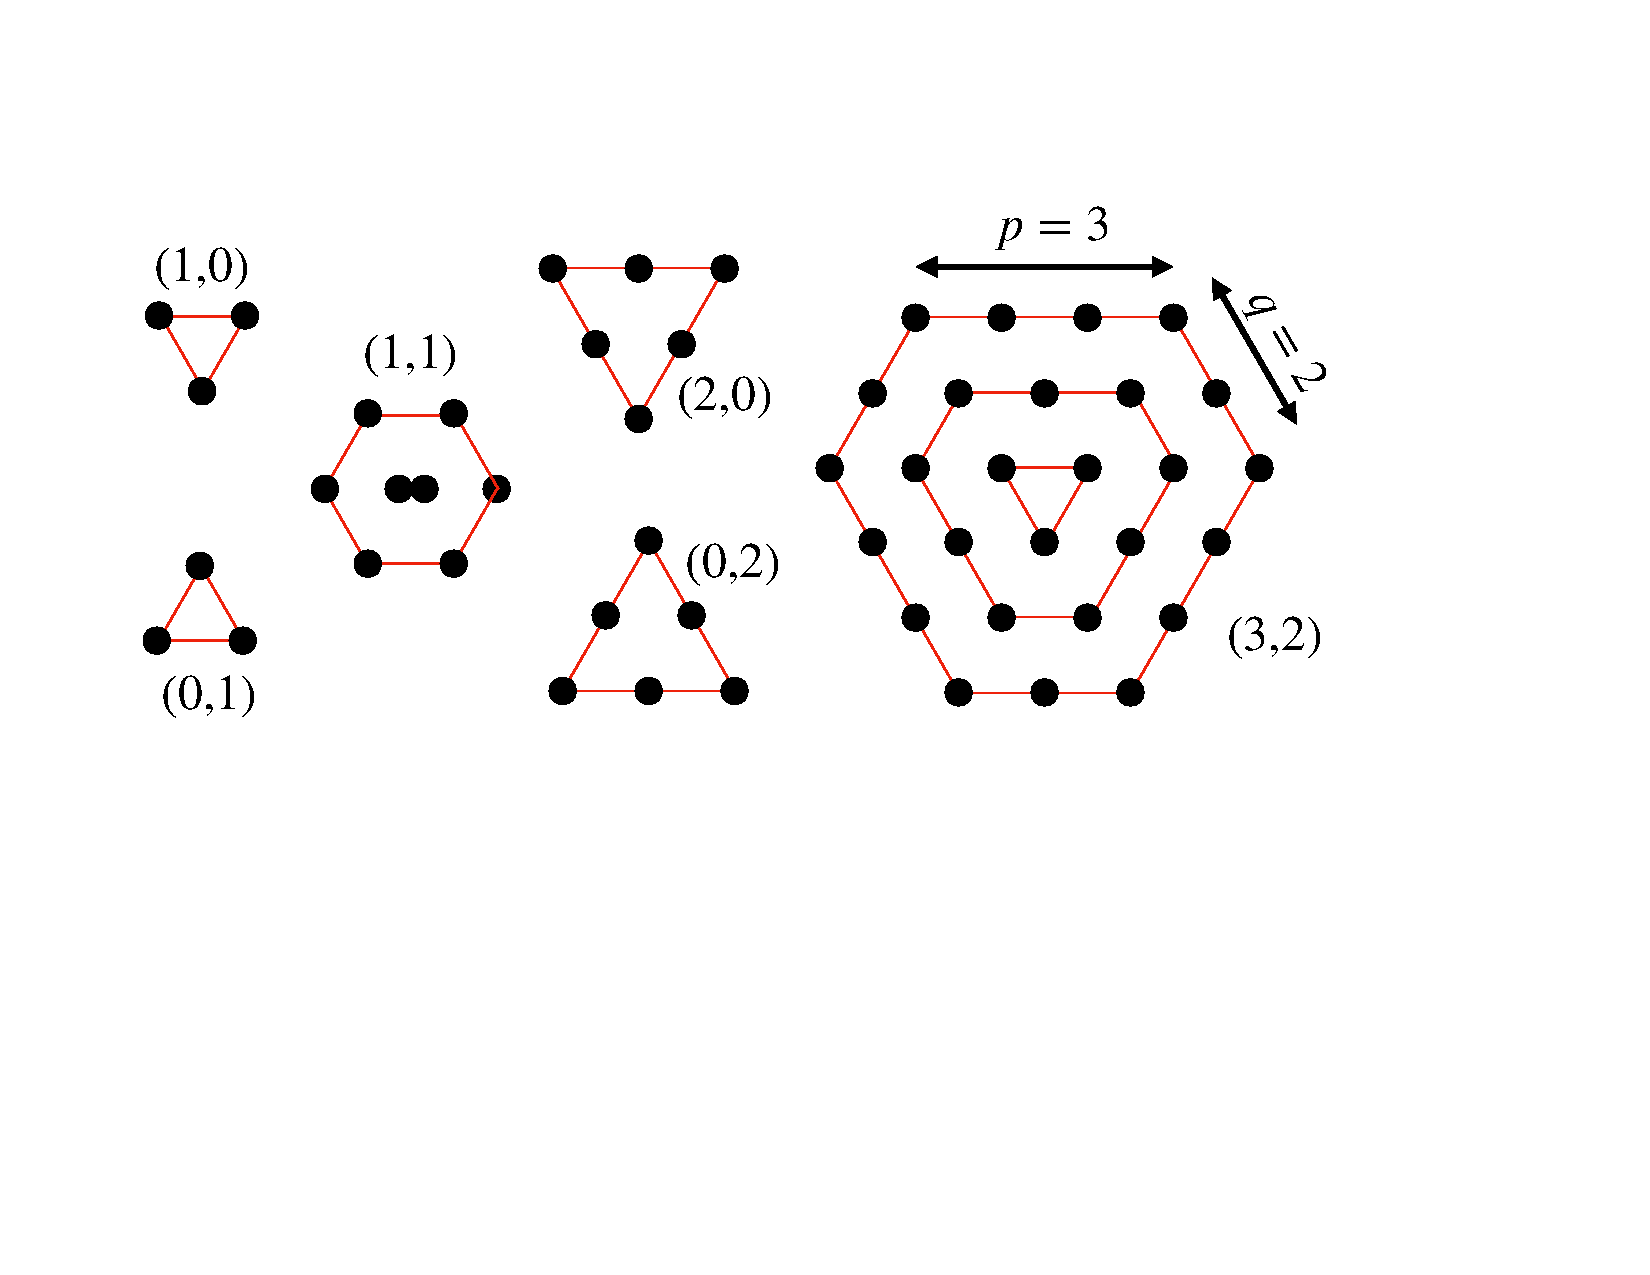
\includegraphics[width=0.6\textwidth]{figs/pqmultiplet.pdf}}
\caption{\label{fig:pqmultiplet}
Graphical representation of $(p,q)$ multiplets. The quark and antiquark color{} triplets are represented by $(1,0)$ and $(0,1)$, respectively, while the gluon octet is $(1,1)$. Each dot represents one projection of the multiplet, if the dot is on the outer ring. Subsequently, for the next inner-ring ring a dot represents two states, or three states for the next inner-ring, although the increasing degeneracy stops once a ring has either $p=0$ or $q=0$. The net degeneracy of the multiplet is $(p+1)(q+1)(p+q+2)/2$. In SU(2) one can combine multiplets of $j_1$ and $j_2$ to form several multiplets $j'$. Similarly, in SU(3) one can combine multiplets of $(p_1,q_1)$ and $(p_2,q_w)$ to form multiplets of several combinations of $(p',q')$.
}
\end{figure}

....

\begin{figure}
\centerline{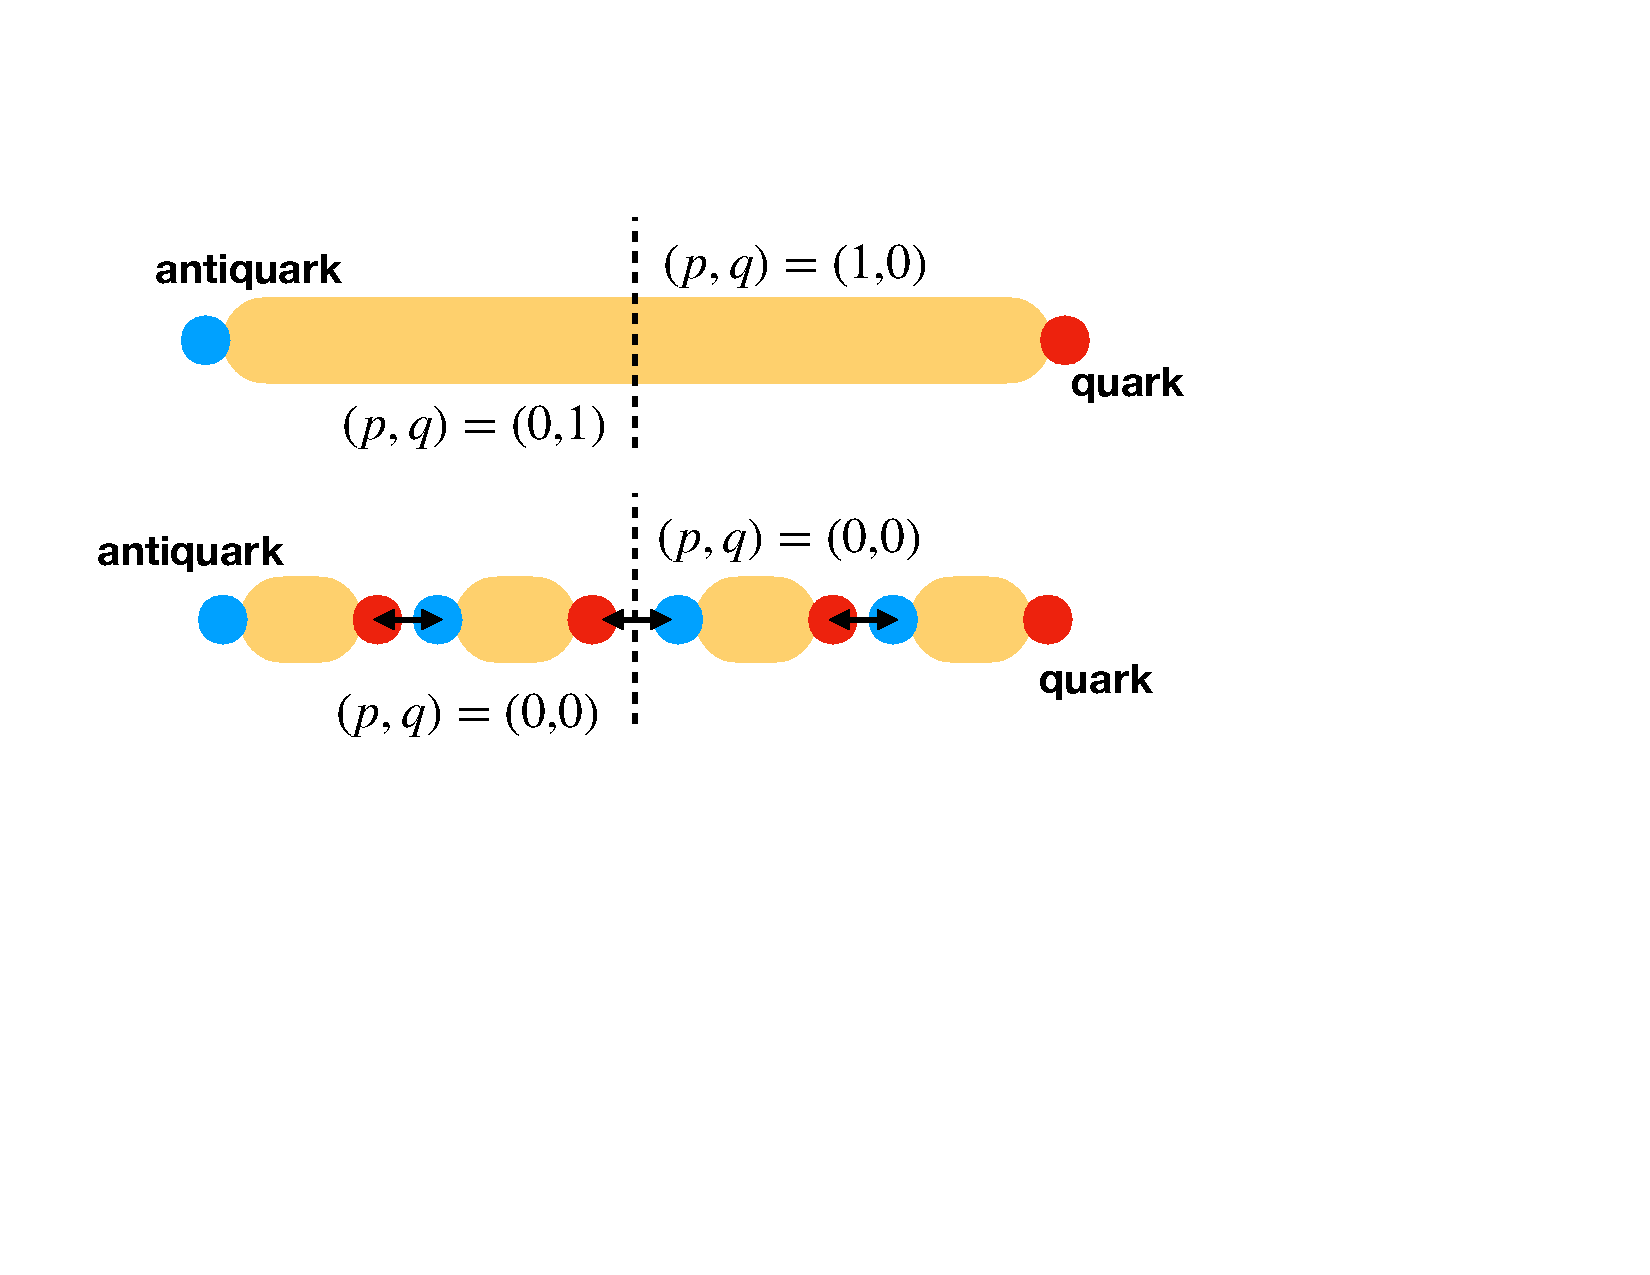
\includegraphics[width=0.5\textwidth]{figs/simpletube.pdf}}
\caption{\label{fig:simpletube}
A simple flux tube between a quark $(p=1,q=0)$ and an antiquark $(p=0,q=1)$ is illustrated in the upper panel, with the lighter and darker circles representing the quark and antiquark respectively. Drawing a vertical line through a flux tube divides space into two regions, the left side of the dashed line in a color multiplet $(p=1,q=0)$ and the right side in the multiplet $(p=0,q=1)$. The lower panel illustrates how quark-antiquark pairs can tunnel out of the vacuum so that the space between the tunneling quarks is free of color fields. Tunneling quark-antiquark pairs are denoted by the arrows.  Dividing space that does not bisect a tube results in both sides being in color singlets.
}
\end{figure}


\begin{figure}
\centerline{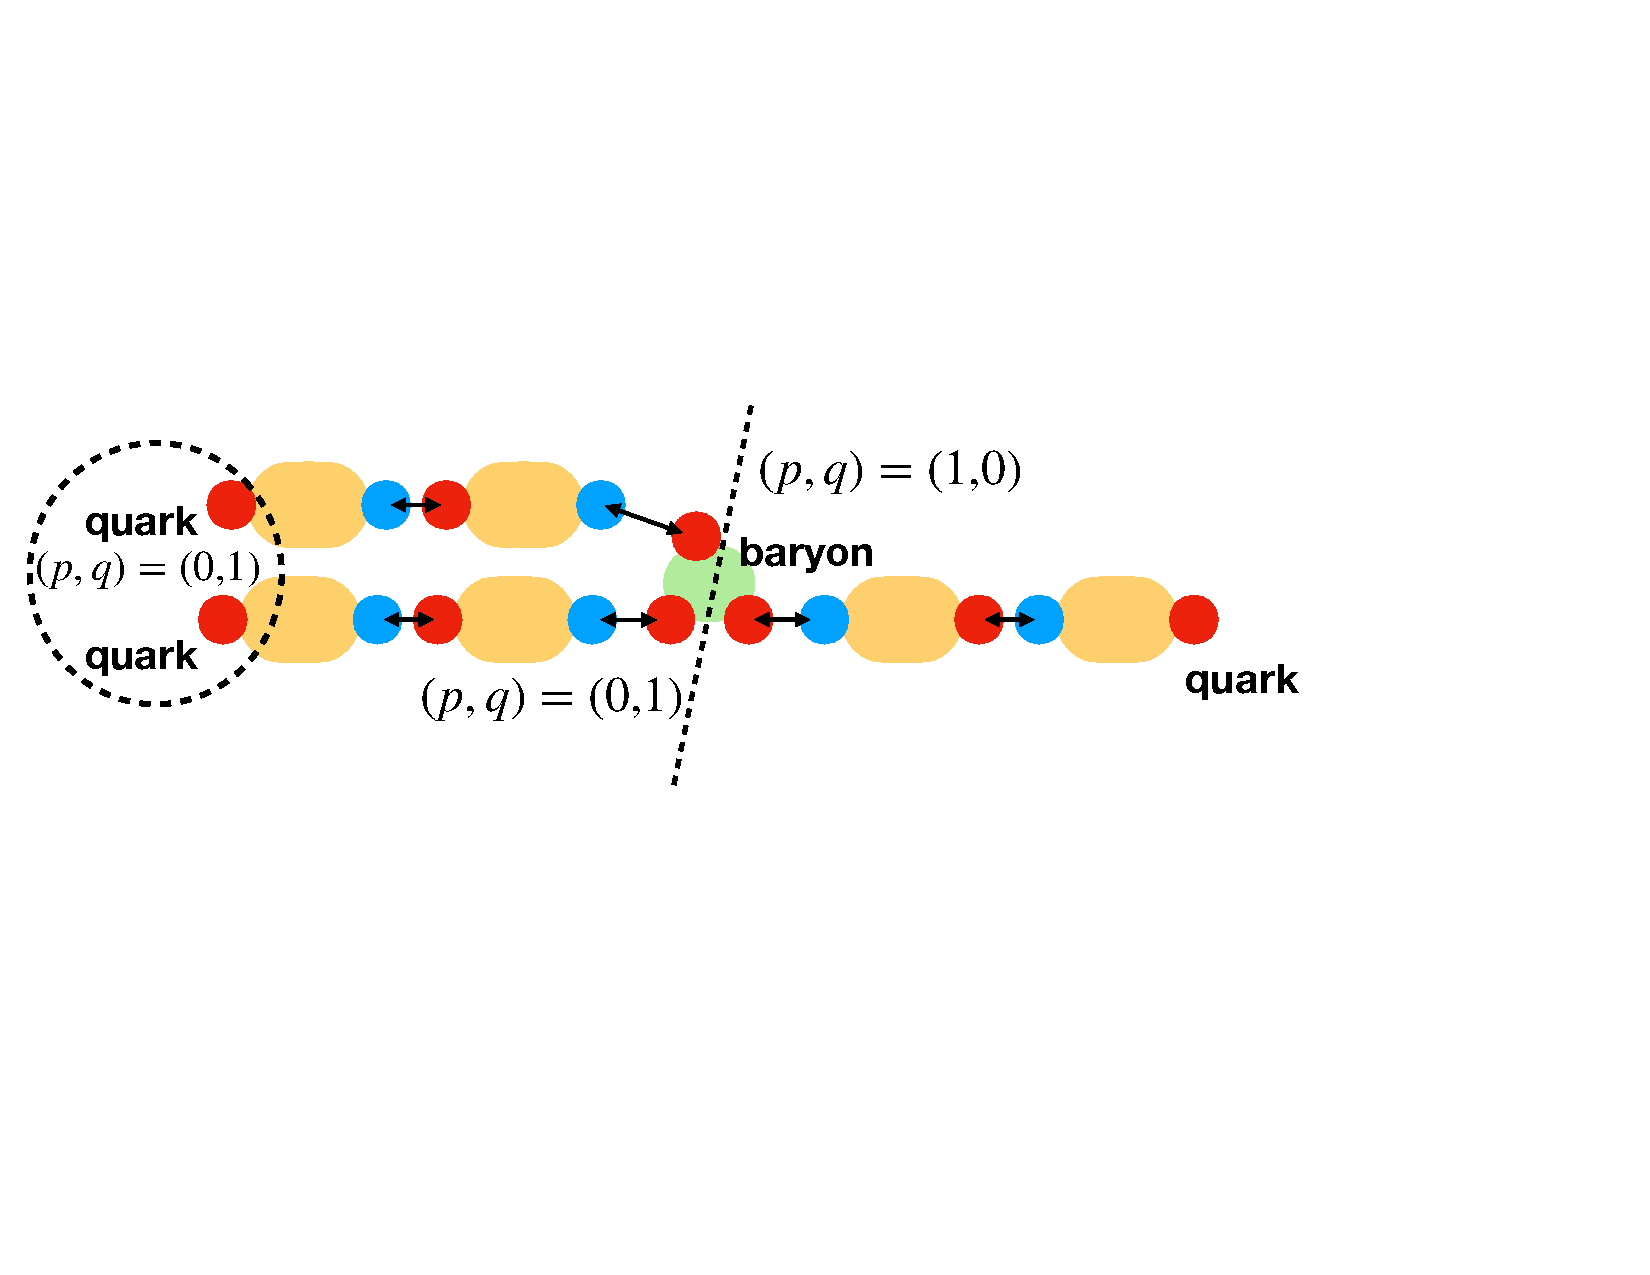
\includegraphics[width=0.6\textwidth]{figs/simplemerge.pdf}}
\centerline{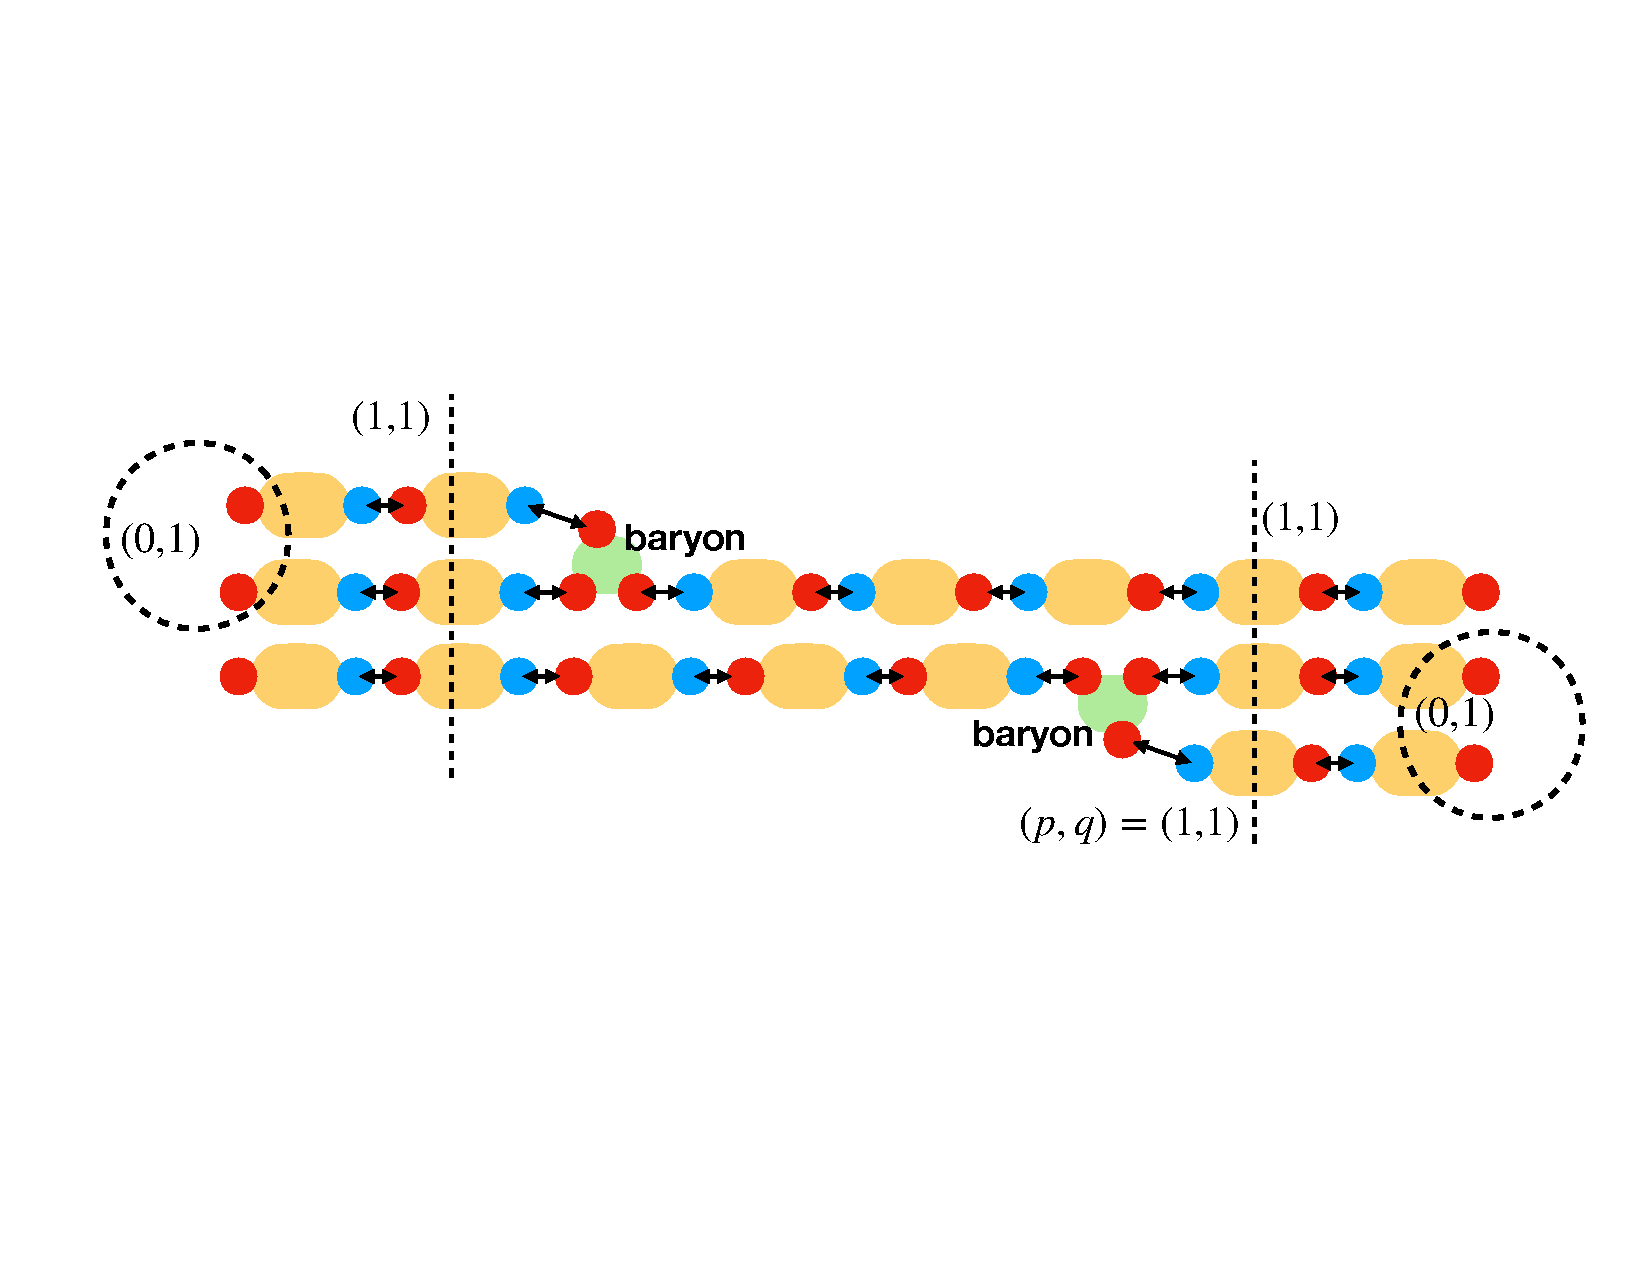
\includegraphics[width=0.9\textwidth]{figs/gluonexchange.pdf}}
\caption{\label{fig:merge}
Upper illustration: The merge of two tubes into one, where the left-hand side tubes begin with two quarks, and the right-hand side ends with one quark. The two quark multiplets couple to a $(0,1)$ multiplet, which then matches with the quark multiplet on the right. The baryon number, is then located at the point where the two tubes merged. This represents a situation where one quark is scattered far, from its original momentum, and the flux tubes must adjust to form local color singlets. The original quark pair must couple to $(p=0,q=1)$ if the overall configuration is to be a color singlet.\\
Lower illustration: This represents the case where two baryons exchange a soft gluon. In that case both of the baryons are transformed into $(p=1,q=1)$ multiplets. Assuming that for each baryon there is a diquark with $(p=0,q=1)$, the overall color singlet is restored by migrating the baryon number to the two places where the strings merge.\\
Darker circles represent quarks, while darker circles represent antiquarks. Ovals represent fluxtubes, and arrows describe quark-antiquark pairs that tunneled from vacuum.
}
\end{figure}


\section{Connecting Baryon Transport to Color Fields}

It is not obvious to see how baryon transport is connected to gluonic fields, $G^{\mu\nu}_a(x)$. Unlike the case for electric fields, gluon fields have a color index, $a$, and because all of nature is in a color singlet, the expectation of the field operators are zero, $\langle G^{\mu\nu}_a(x)\rangle=0$. Therefore, one must describe the fields through operators involving products of operators with color indices. Further, gluons couple to color charge, not to baryon charge. The rather modest goal of this section is to write operators in terms of QCD field operators that represent the baryon polarization and the the field-like operators that drive the polarization. These operators will be discussed in the context of flux tubes. None of the expressions derived here are directly applicable, but the presentation may help elucidate how fields in QCD can inspire baryon movement and separation.

Here, the color electric/magnetic field operators and the color current operators will be considered, $G^{\mu\nu}_a(x)$, and $j^\mu_a(x)$. Instead of the usual definition of such operators, we add an additional feature that enables the construction of gauge-invariant correlators. For any operator $\mathcal{O}(x)$, an additional attached operator is inferred \cite{Elze:1989un},
\begin{eqnarray}
\mathcal{O}_a(x)&\rightarrow \exp\{i\mathcal{P}\int d\vec{\ell}\cdot\vec{A}\}\mathcal{O}_a(x)\mathcal{P}\exp\{ig\int d\vec{\ell}\cdot\vec{A}\}.
\end{eqnarray}
Here, $\mathcal{P}$ is the path-ordering operator. With this definition, if some correlator $\langle\mathcal{O}_a(x)\mathcal{O}_a(x)\rangle$ is gauge invariant, then $\langle\mathcal{O}_a(x)\mathcal{O}_a(y)\rangle$ is also gauge invariant, though one needs to realize that the new correlator might depend on the actual path chosen. With this definition, one can write expressions that appear similar to those for Maxwell's equations,
\begin{eqnarray}
\partial_\mu j^\mu_a(x)&=&0,\\
\nonumber
\partial_\mu G^{\mu\nu}_a(x)&=&j^\nu_a(x).
\end{eqnarray}
Because all observables must be invariant to rotations in color space, one knows that $\langle\mathcal{O}_a\rangle=0$ and one must consider only colorless correlators. To find quantities which can be treated, at least to some degree, similarly as fields, we consider the following operators defined in terms of operators $j_a^\mu(x)$, where $a$ is a color index. 
\begin{eqnarray}
Q_{a,\Omega}&=&\int d\Omega_\mu j^{\mu}_a(x),\\
\nonumber
\langle Q^{(2)}_{\Omega_1,\Omega_2}\rangle&=&\int d\Omega_{1,\mu}\Omega_{2,\nu}\langle j^\mu_a(x_1) j^\nu_a(x)\rangle,\\
\nonumber
&=&\langle Q_{a,\Omega_1}Q_{a,\Omega_2}\rangle,\\
\nonumber
\langle j^{(2)\nu}_{\Omega_1}(x)\rangle &=&\int d\Omega_{1,\mu} \langle j^\mu_a(x_1) j^\nu_a(x)\rangle\\
\nonumber
&=&\langle Q_{a,\Omega_1}j^\nu_a(x)\rangle.
\end{eqnarray}
Here, the superscripts $(2)$ reference the fact that these correlations are quadratic in the color charge. The volumes $\Omega_1$ and $\Omega_2$ can be any chosen volumes. If the volumes cover all space, and if the system is in an overall color singlet, $Q^{(2)}=0$. One can also define correlators using the fields,
\begin{eqnarray}
\langle G^{(2)\mu\nu}_{\Omega}(x)\rangle&=&\int d\Omega_1\langle Q_{a,\Omega}G^{\mu\nu}_a(x)\rangle.
\end{eqnarray}

\begin{acknowledgments}
This work was supported by the Department of Energy Office of Science through grant number DE-FG02-03ER41259.
\end{acknowledgments}

\input biblio.tex

\end{document}
